\section{Datasets and Experimental Setup}
\label{sec:data}

\begin{figure}[!t]
\centering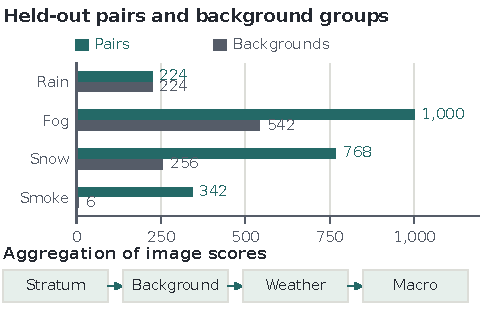
\includegraphics[width=\linewidth]{figures/benchmark_protocol.pdf}
\caption{Test coverage and aggregation. The 342 smoke pairs come from six backgrounds. Image scores are averaged within strata and then across strata, backgrounds, and weather conditions with equal weights at each level.}
\label{fig:benchmark-protocol}
\end{figure}

\begin{figure*}[t]
\centering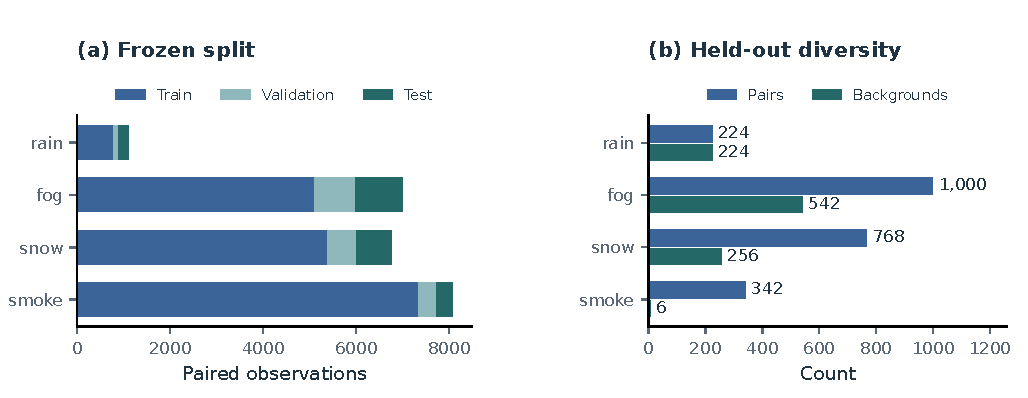
\includegraphics[width=\linewidth]{figures/dataset_coverage.pdf}
\caption{Completed data preparation: the frozen train/validation/test mixture and the distinction between held-out pairs and backgrounds. Smoke's many paired observations cover only six test backgrounds. Counts come from the saved split table.}
\label{fig:dataset-coverage}
\end{figure*}
\paragraph{Paired data.}
The active mixture combines processed real-rain pairs from RealRain-1k-H~\cite{Li_2022_RealRain}, synthetic haze from RESIDE-6K as a fog proxy, SnowCityscapes synthetic snow, and surveillance smoke from a repaired SmokeBench~\cite{Jin_2025_SmokeBench} partition. The source datasets supply all weather effects. Table~\ref{tab:data} and Fig.~\ref{fig:dataset-coverage} report the frozen split, including background groups. Figure~\ref{fig:benchmark-protocol} relates test coverage to the aggregation rule.

\begin{table}[!t]
\centering\small\setlength{\tabcolsep}{4pt}
\caption{Active paired split. Parentheses give background groups, which may contain related observations.}
\label{tab:data}
\begin{tabular}{@{}lrrr@{}}\toprule
Source & Train & Val. & Test\\\midrule
RealRain-1k-H &773 (755)&112 (112)&224 (224)\\
RESIDE-6K &5,102 (5,061)&897 (893)&1,000 (542)\\
SnowCityscapes &5,382 (1,794)&618 (206)&768 (256)\\
SmokeBench &7,353 (31)&384 (6)&342 (6)\\\midrule
Total pairs &18,610&2,011&2,334\\\bottomrule
\end{tabular}
\end{table}

A decode audit of 52,140 active and reserve files finds zero exact cross-split overlaps or near-target candidates under the specified thumbnail and pHash rule. The repaired split removes the identified smoke-reference overlap. Reserved snow/smoke pairs stay excluded from selection and testing. Sequence independence and alignment remain imperfectly characterized. Appendix~\ref{app:data} gives the audit thresholds and reserve counts.

\paragraph{Aggregation.}
For per-image RGB PSNR or SSIM $m_i$, let $I_s$ be images in stratum $s$, $S_g$ strata for background $g$, and $G_w$ backgrounds for weather $w$. We report
\begin{equation}
\bar m=\frac14\sum_w\frac1{|G_w|}\sum_{g\in G_w}
\frac1{|S_g|}\sum_{s\in S_g}\frac1{|I_s|}\sum_{i\in I_s}m_i.
\label{eq:metric}
\end{equation}
Strata rank thumbnail input/target differences within each background as a degradation proxy. Equal weighting at each level limits the influence of many variants from a single scene. Evaluation uses native-resolution BF16 forward passes and RGB in $[0,1]$, with MSE floor $10^{-12}$ and uniform $7\times7$ sample-covariance SSIM. Metrics precede 8-bit export. All 14,004 model/image rows support reaggregation. Cluster resampling estimates uncertainty conditional on these checkpoints and test groups.

\subsection{Training, validation and test responsibilities}
The sampler draws 4,096 pairs per epoch with replacement; this is not a pass
through all 18,610 training pairs. With global batch four, a 60-epoch run has
61,440 optimizer steps. Paired cropping and flipping preserve correspondence
between input and target. At evaluation, native images are padded as required
by the model and cropped back before scoring. The best validation macro PSNR
selects a checkpoint; the test partition supplies the reported comparison.

The 0.30/0.30/0.30/0.10 weather probabilities describe training draws.
They are independent of the equal-weather averaging used at evaluation.
Changing either sampling or aggregation changes the experimental question.
The fixed active manifest is therefore preserved rather than reconstructed
for this report.

\subsection{Metrics and uncertainty}
For $N$ RGB samples in $[0,1]$, the per-image peak signal-to-noise ratio is
\begin{equation}
\operatorname{PSNR}(y,\hat y)=10\log_{10}\!\left(\frac{1}{\max(\operatorname{MSE}(y,\hat y),10^{-12})}\right).
\end{equation}
The finite MSE floor prevents infinities in serialized outputs. SSIM uses
uniform $7\times7$ windows, sample covariance and the same unit data range.
The benchmark averages image-level scores hierarchically; it does not compute
PSNR from a pooled pixel MSE. Output comparisons for export use a separate
normalized tensor domain, described in Section~\ref{app:quant}.

The cluster bootstrap uses 2,000 resamples of the recorded test groups while
holding trained checkpoints fixed. It estimates conditional test uncertainty,
not variability across training seeds. There is one seed per system. The
six-model runs also use different pretrained starting weights, so the results
cannot isolate the causal effect of architecture from prior data exposure.

\subsection{Hardware and experimental domains}
Training uses BF16 on an NVIDIA A100-SXM4-40GB; the continuation study uses
two A100s with the same global batch. Native test inference uses BF16, while
the saved qualitative examples and local resolution diagnostics use CPU FP32.
The later on-device study uses the original 4\,GB Nano with L4T 32.7.3,
Python 3.6.9 and TensorRT 8.2.1.8. These domains are reported separately
because neither numerical agreement nor native-resolution quality can be
assumed to transfer unchanged across canvases and runtimes.
